\documentclass[12pt,a4paper]{ctexart}

% 导入必要的宏包
\usepackage{geometry}
\usepackage{graphicx}
\usepackage{amsmath}
\usepackage{amssymb}
\usepackage{xcolor}
\usepackage{enumitem}
\usepackage{titlesec}
\usepackage{fancyhdr}
\usepackage{booktabs}
\usepackage{multirow}
\usepackage{caption}
\usepackage{float}

% 页面设置
\geometry{left=2.5cm,right=2.5cm,top=2.5cm,bottom=2.5cm}

% 标题格式设置
\titleformat{\section}{\Large\bfseries}{\chinese{section}、}{0.5em}{}
\titleformat{\subsection}{\large\bfseries}{\arabic{subsection}.}{0.5em}{}

% 页眉页脚设置
\pagestyle{fancy}
\fancyhf{}
\fancyhead[C]{流光守护智能夜跑服设计报告}
\fancyfoot[C]{\thepage}

% 文档信息
\title{\textbf{``流光守护''智能夜跑服设计报告}}
\author{}
\date{\today}

\begin{document}

\maketitle
\thispagestyle{empty}

\vspace{1cm}

\section{设计背景与目标}

全民健身理念兴起，多数人选择夜间跑步。针对传统反光服饰被动受光的局限，本设计提出``流光守护''智能夜跑服。利用QD-LED（量子点发光二极管）技术实现主动发光，提升运动者在复杂路况下的识别度与安全性。

\section{器件选择与深度设计}

\subsection{需求分析与指标设计}

针对夜跑场景，器件需满足：高可见度亮度（亮度 > 1000 cd/m²）、色彩高纯度、低驱动电压（<4V）及卓越柔韧性。

\subsection{材料选择}

\subsubsection*{发光材料}

选用环保型InP/ZnS结构量子点。相比传统的镉系量子点，其环境友好性更高且荧光量子产率（PLQY）可达90\%以上，确保高效发光。

\subsubsection*{传输层材料}

电子传输层（ETL）选用纳米ZnO溶液，空穴传输层（HTL）选用TFB或PVK有机聚合物。这种``无机+有机''的杂化组合能有效平衡载流子注入，提升器件外量子效率（EQE）。

\subsubsection*{柔性衬底}

选用TPU薄膜柔性衬底，确保器件在运动拉伸时不易失效。

\subsection{器件结构选择}

采用倒置器件结构（Inverted Structure），即``衬底/ITO/ZnO/QD/HTL/金属阳极''。该结构相较于正置结构具有更强的空气稳定性，且更易于进行大面积的封装保护。

\begin{figure}[H]
    \centering
    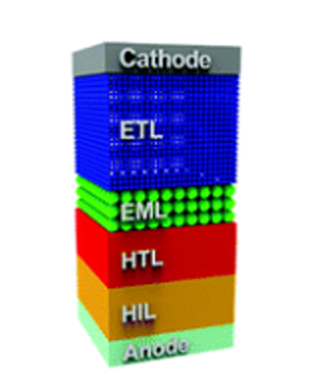
\includegraphics[width=0.4\textwidth]{p1.png}
    \caption{QD-LED器件层级结构示意图}
    \label{fig:structure}
\end{figure}

\begin{table}[H]
    \centering
    \caption{QD-LED各层级材料选择与设计逻辑}
    \label{tab:layers}
    \small
    \begin{tabular}{cccp{5.5cm}}
        \toprule
        \textbf{图片层级} & \textbf{对应名称} & \textbf{推荐材料} & \textbf{核心逻辑} \\
        \midrule
        顶部 & Cathode（阴极） & 金属阳极（Al/Ag） & 倒置结构顶电极，兼顾导电性与空气稳定性 \\
        第二层 & ETL（电子传输层） & 纳米ZnO溶液 & 无机材料，提供优异的电子注入效率与稳定性 \\
        第三层 & EML（发光层） & InP/ZnS核壳结构量子点 & 环保无镉，PLQY $>$ 90\%，确保高效多色发光 \\
        第四/五层 & HTL/HIL（空穴层） & TFB或PVK有机聚合物 & 优化空穴传输，实现载流子注入平衡，提升EQE \\
        底部 & Anode（阳极） & ITO柔性透明电极 & 结合PI/TPU柔性衬底，保证高透光率与耐弯折性 \\
        \bottomrule
    \end{tabular}
\end{table}

\subsection{制造工艺选择}

采用溶液法（Solution Processing）中的喷墨打印技术（Inkjet Printing）。该工艺不仅材料利用率高，且能实现在柔性衬底上的图案化精密布线，支持个性化流光纹路设计。

\subsection{织物集成工艺}

选择高弹、透气的聚酯纤维与氨纶混纺织物作为基材。利用\textbf{热压复合技术（Thermal Bonding）}将封装好的柔性QD-LED模块嵌入服装层间，配合纳米防水涂层，解决排汗与洗涤对电路的影响。

\section{综合评估}

\subsection{成本与可行性}

溶液加工工艺规避了高能耗的真空蒸镀，显著降低量产成本。随着柔性电子产业链成熟，工艺可行性极高。

\subsection{环境与社会效益}

采用无镉材料符合绿色环保标准；产品显著降低了夜间交通事故率，具有极强的公共安全保障价值与市场前景。

\end{document}
